\documentclass[11pt,a4paper]{article}

\usepackage{fullpage}
\usepackage{hyperref}
\usepackage{graphicx}
\usepackage{enumerate}
\usepackage{tikz}
\usepackage{amsmath}
\usepackage[bottom]{footmisc}
\usetikzlibrary{shapes, arrows, positioning, fit, backgrounds}
\usepackage{color}
\definecolor{pblue}{rgb}{0.13,0.13,1}
\usepackage{listings}
\lstset{language=Java,
		keywordstyle=\color{pblue},
		 breaklines=true,
		 basicstyle=\small,
		 tabsize=2
}
\usepackage{fancyhdr}
\pagestyle{fancy}
\fancyhf{}

\renewcommand{\headrulewidth}{0pt}
\renewcommand{\footrulewidth}{0pt}

\fancypagestyle{firstpagefooter} {
	\lfoot{\tiny{Version: 02.12.2017}}
	\cfoot{}
	\rfoot{\thepage}
	
}

\lfoot{Name: Simon Haefeli , Legi: 13-918-107}
\rfoot{\thepage}

\begin{document}

\title{Advanced Systems Lab Report\\ \normalsize{Autumn Semester 2017}}
\author{Name: Simon Haefeli\\Legi: 13-918-107}
\date{
	\vspace{4cm}
	\textbf{Grading} \\
	\vspace{0.5cm}
	\begin{tabular}{|c|c|}
		\hline  \textbf{Section} & \textbf{Points} \\
		\hline  1                &                 \\ 
		\hline  2                &                 \\ 
		\hline  3                &                 \\ 
		\hline  4                &                 \\ 
		\hline  5                &                 \\ 
		\hline  6                &                 \\ 
		\hline  7                &                 \\ 
		\hline \hline Total      &                 \\
		\hline 
	\end{tabular} 
}
\maketitle
\thispagestyle{firstpagefooter}

\newpage


\section{System Overview}
\subsection{Abstract}
This project consisted of designing, implementing and evaluating the performance of a key-value store network system. We added a so-called middleware between the memtier benchmark clients and the memcached servers that was able to forward the requests and answers and do some processing for certain particular requests. In this report, we first discuss the way the middleware was implemented, then we analyze results of different experiments and finally model our system.\footnote{To get an overview of the files of this project, please refer to the README, found at the root of the project} 
\subsection{General design and implementation particularities}
Even though the general structure of the middleware was clearly defined, the components of the middlware asked for some important design choices. What follows below is a small overview of the different implementation choices. 

\begin{center}
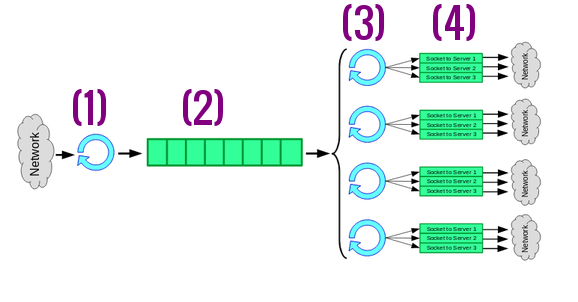
\includegraphics[scale=0.69]{baseIm.png}
\end{center}
\begin{enumerate}[ {(}1{)} ]
\item The net thread is the thread that accepts connections from the clients, and reads the incoming requests to put them in the request queue (2). The \textit{Java.nio} (non-blocking IO) package was used to achieve this purpose: a \textit{ServerSocketChannel} was used as a welcome socket to accept connections from the clients by creating for each client a \textit{SocketChannel}, and a \textit{Selector} was used to iterate over the sockets (the connection sockets and the welcome socket) to find entering requests for the middleware or connection requests. Using \textit{Java.nio} allows us not only to abstract the handling of a various number of connections, but also it iterates over the client connections in an optimal way by using \textit{SelectionKeys}. 
\item The request queue is a java \textit{LinkedBlockingQueue}, which has the useful properties to be unbounded and be FCFS\footnote{First come first serve}. Requests wait in this queue until a worker thread is free.   

\item The request queue and the worker threads are both managed by the java \textit{ThreadPoolExecutor}. The thread pool executor, which definition is: 
\begin{lstlisting}
	ThreadPoolExecutor(int corePoolSize, int maximumPoolSize, long keepAliveTime, TimeUnit unit, LinkedBlockingQueue workQueue)
\end{lstlisting} 
has a fixed number of worker threads by setting corePoolSize = maximumPoolSize. Putting a request into the queue or executing it, depending on the availability of the worker threads, is being done by the same following instruction:
\begin{lstlisting}
	myThreadPoolExecutor.execute(Runnable command)
\end{lstlisting}
The \textit{ThreadPoolExecutor} will execute the command if a worker thread is available, or put it to the unbounded queue if not, which is exactly the expected behaviour.\footnote{https://docs.oracle.com/javase/7/docs/api/java/util/concurrent/ThreadPoolExecutor.html, part on "Queuing"}     
 
\item The connection sockets with the memcached servers are normal Java sockets, from the \textit{Socket} class. Each worker thread opens a socket to each memcached server the first time it is beeing run and keeps it open until the middleware is stopped.  
\end{enumerate}

\subsection{Request handling}
We now take a closer look at the implementation of the middleware and how the pipeline looks like for a request being processed. The following flow chart illustrates this:
\\
\\\\
% Define block styles]
\tikzstyle{block} = [rectangle, draw, fill=blue!20, 
    text width=9em, text centered, rounded corners, minimum height=4em]
\tikzstyle{line} = [draw, -latex']
\tikzstyle{cloud} = [draw, ellipse,fill=red!20, node distance=3cm,
    minimum height=2em]   
\begin{tikzpicture}[node distance = 3cm, auto]
    % Place nodes
    \node [block] (RunMW) {\textbf{\underline{RunMW}} \\ \textit{main(): starts the mw}};
    \node [block, below=0.7cm of RunMW] (MyMiddleware) {\textbf{\underline{MyMiddleware}} \\ \textit{run(): reads the text from the socket and creates a prerequest}};
    \node [block, left=3cm of MyMiddleware, text width=8em] (Params) {\underline{static Params} \\ inputs predefined parameters};
    \node [block, right=2cm of MyMiddleware] (PreRequest) {\textbf{\underline{PreRequest}} \\ \textit{PreRequest(): creates an object with the text and a starting time}};
    \node [block, below of=MyMiddleware] (QueueHandler) {\textbf{\underline{QueueHandler}} \\ \textit{putToQueue(): calls the threadPoolExecutor execute function on the Prerequest}};
    \node [block, left=3cm of QueueHandler, text width=11em] (StatisticsAggregator) {\textbf{\underline{StatisticsAggregator}} \\ \textit{run(): Gets statistics from different classes every time window, processes and stores them in the Statistics class}};
     \node [block, below of=StatisticsAggregator, text width=8em] (Statistics) {\underline{static Statistics} \\ Contains the aggregated statistics};
      \node [block, below=1cm of QueueHandler] (RequestHandler) {\textbf{\underline{RequestHandler}} \\ \textit{run(): creates a Request to parse the PreRequest and calls the appropriate handling function}};
      \node [block, right=2cm of RequestHandler, text width=8em] (Request) {\textbf{\underline{Request}} \\ \textit{Request(): parses the text received from the client with the correct RequestType}};
      \node [block, above of=Request] (RequestType) {\underline{static RequestType} \\ Contains the different request types};
      \node [cloud, below=0.8cm of RequestHandler] (HandleGet) {HandleGet()};
      \node [cloud, right=0.5cm of HandleGet] (HandleSet) {HandleSet()};
      \node [cloud, left=0.5cm of HandleGet] (HandleMGet) {HandleMGet()};
      
    % Draw edges
    \path [line] (RunMW) -- (MyMiddleware);
    \draw[>=latex,->] ([yshift= -5pt] PreRequest.west) -- ([yshift= -5pt] MyMiddleware.east);
    \draw[>=latex,<-] ([yshift= 5pt] PreRequest.west) -- ([yshift= 5pt] MyMiddleware.east);
  
    \path [line] (Params) -- (MyMiddleware);
    \path [line, dashed] (MyMiddleware) -- (StatisticsAggregator);
    \path [line, dashed] (QueueHandler) -- (StatisticsAggregator);
    \path [line, dashed] (RequestHandler) -- (StatisticsAggregator);
    \path [line] (StatisticsAggregator) -- (Statistics);
    \path [line] (MyMiddleware) -- (QueueHandler);
    \path [line] (QueueHandler) -- (RequestHandler);
    \draw[>=latex,->] ([yshift= 5pt] RequestHandler.east) -- ([yshift= 5pt] Request.west);
    \draw[>=latex,<-] ([yshift= -5pt] RequestHandler.east) -- ([yshift= -5pt] Request.west);
    \draw[>=latex,<-] ([xshift= 5pt] Request.north) -- ([xshift= 5pt] RequestType.south);
    \draw[>=latex,->] ([xshift= -5pt] Request.north) -- ([xshift= -5pt] RequestType.south);
    \path [line] (RequestHandler) -- (HandleMGet);
    \path [line] (RequestHandler) -- (HandleGet);
    \path [line] (RequestHandler) -- (HandleSet);
\end{tikzpicture}
\\\\
To make some correpondences with the general structure of the middleware presented in section 1.2, we see that the \textit{MyMiddleware run()} function represents the net thread, the \textit{QueueHandler} class has a \textit{ThreadPoolExecutor} field that manages the request queue and the call of the worker thread, and that the \textit{RequestHandler run()} function represents one worker thread. We may also note that a PreRequest class is created before putting the received message into the queue. This is done to bind the message with a time point and to be able to track the time a message spends in the queue. 
\\\\
At the end of the pipeline, the different requests are treated according to their type (get, set, or multi-get). In case of a set, the request is sent to all memcached servers sequentially, after what the worker thread waits for all the answers, also sequentially, as showed in the next line in the case of 3 memcached servers. 
\begin{lstlisting}
	1				send to server 1
	2				send to server 2
	3				send to server 3
	4				wait for answer 1 until received
	5				wait for answer 2 until received
	6				wait for answer 3 until received
	7				merge the answers and send back to client
\end{lstlisting}
The main drawback of this design is that if one of the servers has a higher latency than the other ones, the worker thread might be waiting idly instead of starting to read the answers from the other servers. 
\\
In case of a get request, we simply forward the request to a given server. To decide to which memcached server we send the request, we simply keep a static field in the \textit{RequestHandler} class which is shared accross the worker threads and which keeps track of the last server to which we sent a get request. This variable is then updated in a round-robin way. 
\\
In case of a multi-get, two cases are possible: In the non-sharded case, the request is simply being executed as a normal get. In the sharded case, the multi get is beeing splitted equally accross the different available memcached servers.   
\\\\
Finally, since we want the connections between the middleware and the servers to be open before running the experiments, we need to initialize these once for every worker thread. By defining the connection sockets with the servers in a \textit{ThreadLocal} in the \textit{RequestHandler} class, the initialization of the sockets will happen only the first time a worker thread is beeing called. That's why every thread is called once during the initialization phase of the middleware, by executing number of worker threads times the "init" requests, which are fake requests that do not need any special handling.\footnote{According to the javadoc of the ThreadPoolExecutor class, "When a new task is submitted in method execute(java.lang.Runnable), and fewer than corePoolSize threads are running, a new thread is created to handle the request, even if other worker threads are idle". And that's why it is enough to run corePoolSize number of requests to have them run all once and thus initialized their sockets.} 

\subsection{Statistics gathering}
Statistics have to be made in different classes accross the middleware, either a count (number of gets, number of sets,...), or an average (queue length, time in queue,...). These statistics are stored in static atomic fields in the respective classes that can be retrieved from the \textit{StatisticsAggregator} class which is a \textit{Runnable} called every second, the first time at initialization of the middleware. These statistics are then collected every given time window, averaged and stored in the \textit{Statistics} class. This process is illustrated in the next figure:
\\
% Define block styles]
\tikzstyle{block} = [rectangle, draw, fill=green!20, 
    text width=36em, text centered, rounded corners, minimum height=4em]
\tikzstyle{line} = [draw, -latex'] 
\begin{tikzpicture}[node distance = 3cm, auto]
    % Place nodes
      \node [block, text width=36em] (StatisticsAggregator) {\textbf{\underline{StatisticsAggregator}} \\\begin{lstlisting}
	public void run(){
		int timesInQueue = Requesthandler.timesInQueue.getAndSet(0);
		int timesInQueueCount = Requesthandler.timesInQueueCount.getAndSet(0);
		Statistics.queueTimes.add(timesInQueue/timesInQueueCount);
	}
\end{lstlisting}};
    \node [block,text width=31em, below=6cm of StatisticsAggregator.west, anchor=west] (RequestHandler) {\textbf{\underline{RequestHandler}} \\\begin{lstlisting}
	public static AtomicInteger timesInQueue = 0;
	public static AtomicInteger timesInQueueCount = 0;
	public void handleRequest(request){
		ellapsedTime = System.nanoTime()-request.startTime;
		timesInQueue.getAndAdd(ellapsedTime);
		timesInQueueCount.getAndIncrement();
	}
\end{lstlisting}};
    \node [block, right=9cm of RequestHandler.north, anchor=north, text width = 10em] (Statistics) {\underline{Statistics} \\\begin{lstlisting}
	List<Integer> queueTimes;
\end{lstlisting}};
      
    % Draw edges
    \path [line] (StatisticsAggregator) -| (Statistics);
    \draw[>=latex,->] ([xshift= -5pt] RequestHandler.north) -- ([xshift= -5pt] StatisticsAggregator.south);
    \draw[>=latex,<-] ([xshift= 5pt] RequestHandler.north) -- ([xshift= 5pt] StatisticsAggregator.south);

\end{tikzpicture}
\\\\
The collected statistics in the \textit{Statistics} class are then filtered, by removing the warm-up time (according to some experiments I made, the middlware needs around 10 seconds to get stable data) and the cool down time (1 second), and removing the zero values that are present before and after the significative values (zeros that occur because of the late start of a memtier client for example or an early stop). 
\\
Finally, when the middleware is shut down, thanks to a shutdown hook, the average and standard deviation of every statistic is being computed and printed to a file. Depending on the experiment, we sometimes also print all the values to construct histograms.
\newpage  
\section{Baseline without Middleware}
The goal of this experiment is to study how the system would perform without the middleware. This part is important to get a better idea of what the performance limitations of the memcached servers and the memtier benchmark clients are, so that we can better judge the impact of the middleware throughout the rest of the experiments. 

\subsection{One Server}

First, we want to analyze the performance evolution of the memcached server, and eventually find its upper-bound in terms of performance. To achieve this, we set up one single memcached server being queried by a various number of clients, for read-only and write-only workloads. More precisely, we run experiments in the following configurations:
\begin{center}
	\scriptsize{
		\begin{tabular}{|l|c|}
			\hline Number of servers                & 1                        \\ 
			\hline Number of client machines        & 3                        \\ 
			\hline Instances of memtier per machine & 1                        \\ 
			\hline Threads per memtier instance     & 2                        \\
			\hline Virtual clients per thread       & [1..32]                  \\ 
			\hline Workload                         & Write-only and Read-only \\
			\hline 
		\end{tabular}
	} 
\end{center}

\subsubsection{Results and explanation}
For a read only workload, we obtain the following plots for the latency and the throughput for one client machine (the plots are very similar than the ones of the other client machines)\footnote{exp2/baseline1/client02inst1\_ratio0:1\_rep3.txt}
\\
\begin{minipage}{0.5\linewidth}
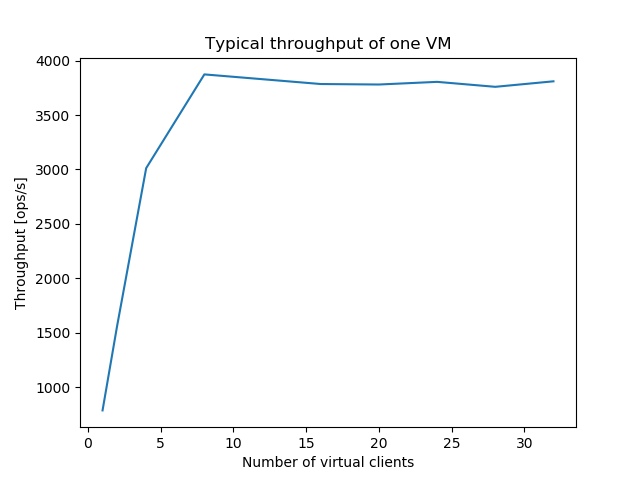
\includegraphics[width=\linewidth]{/home/simon/Documents/ETH/asl/asl-fall17-project/collectedStatFiles/Exp2/baseline1/readOneVMThroughput.png}
\end{minipage}
\hfill
\begin{minipage}{0.5\linewidth}
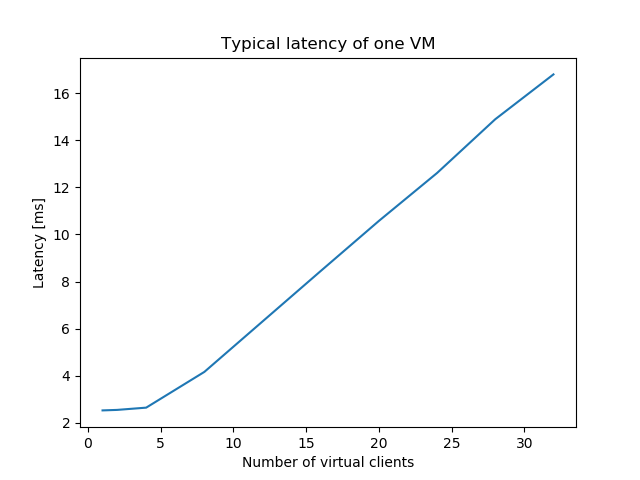
\includegraphics[width=\linewidth]{/home/simon/Documents/ETH/asl/asl-fall17-project/collectedStatFiles/Exp2/baseline1/readOneVMLatency.png}
\end{minipage}
\\\\
We notice that the maximum throughput is already reached with 8 virtual clients per virtual machine and is then stable when we let the number of clients grow. In other words, the memcached server starts to \underline{saturate} when 3 VM with 2 threads and 8 virtual clients are querying a single server simultaneously. It is important to mention here that it is nearly impossible to \underline{over-saturate} a server due to the way the memtier benchmark work: since we always run the clients with the default \textit{--pipeline=1} argument, every CPM\footnote{virtual client per memtier, see project description} will wait for an answer to come back before sending another request.
\\
For the latency, we clearly see that it is inversely proportionnal to the throughput (we distinguish three different slopes on both graphs). In the phase when the number of virtual clients grows at a constant rate (number of virtual clients getting bigger than 8), the throughput also becomes constant. The reason why the throughput does not drop but rather stays at approximately 4000 operations/second even though the latency grows, is because the higher latency is compensated by a higher number of virtual clients to keep the throughput constant. 
\\As a sanity check, we can evaluate the interactive law. Knowing the interactive law is : \[ request Time (w) = \frac{number Of Clients (N)}{throughput (X)}\] and that for example, at 8 virtual clients with two threads in the memtier client, N = 16 and the throughput X is approximately 3800 ops/sec, gives us a response time of 4.2ms, which perfectly corresponds to the previous graphs. This sanity check also works with the remaining results of this experiment. 
\\
For a write-only workload, we obtain the following results:\footnote{exp2/baseline1/client02inst1\_ratio1:0\_rep3.txt}
\\
\begin{minipage}{0.5\linewidth}
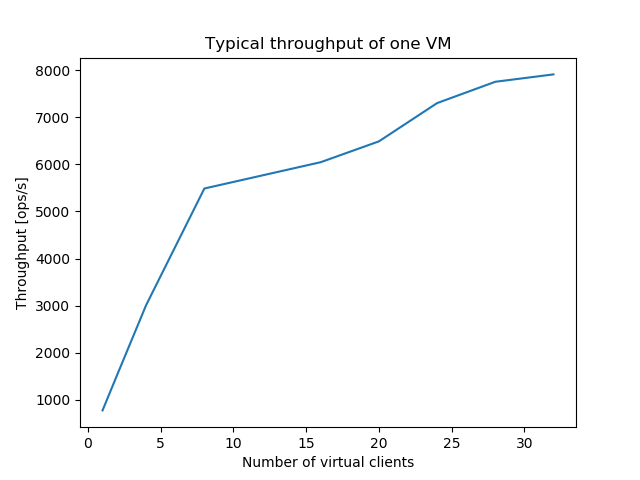
\includegraphics[width=\linewidth]{/home/simon/Documents/ETH/asl/asl-fall17-project/collectedStatFiles/Exp2/baseline1/writeOneVMThroughput.png}
\end{minipage}
\hfill
\begin{minipage}{0.5\linewidth}
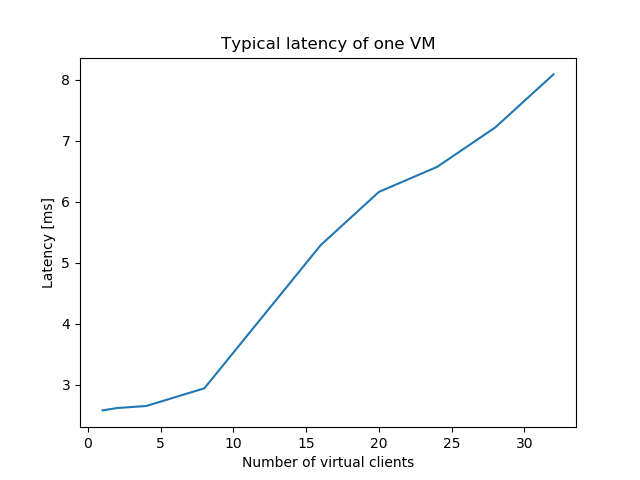
\includegraphics[width=\linewidth]{/home/simon/Documents/ETH/asl/asl-fall17-project/collectedStatFiles/Exp2/baseline1/writeOneVMLatency.png}
\end{minipage}
\\\\\\
For this workload, we note that we barely reach a saturated memcached server with 32 virtual clients, even if there is a clear drop in the growth of the throughput at 8 virtual clients. The observations are made for a read-only workload but they also apply for a write-only workload. 
\\\\
However, we note a maximum throughput twice as high for sets than for gets, with a maximum latency twice as small. The different size of the messages sent back and forth between the clients and the servers may not be the main factor, since for a get the messages are: 
\begin{lstlisting}
	request: get memtier-9999, 		answer: value memtier-9999 XXXXXX
\end{lstlisting}
and for the set they are:
\begin{lstlisting}
	request: set memtier-9999  0 10000 1024 XXXXX,	answer:  STORED
\end{lstlisting}
which are quite the same length. This implies that memcached is either storing values faster than getting values, either sends the \textit{STORED} message back before starting the write operation, that it either has poorer performance than memtier benchmark when writting big messages to the connection sockets, or that it is a combination of these factors. For this report, we will just keep in mind that the achieved throughput is higher with a write-only workload.
   
\subsection{Two Servers}

Now we increase the number of servers and put a single client machine with a single thread to measure the performance limitations of the memtier clients with the following configurations:

\begin{center}
	\scriptsize{
		\begin{tabular}{|l|c|}
			\hline Number of servers                & 2                        \\ 
			\hline Number of client machines        & 1                        \\ 
			\hline Instances of memtier per machine & 2                        \\ 
			\hline Threads per memtier instance     & 1                        \\
			\hline Virtual clients per thread       & [1..32]                  \\ 
			\hline Workload                         & Write-only and Read-only \\
			\hline 
		\end{tabular}
	} 
\end{center}

\subsubsection{Results and explanation}
For a read-only workload, we obtain the following plots:\footnote{exp2/baseline2/client01inst1\_ratio0:1\_rep1.txt and exp2/baseline2/client01inst2\_ratio0:1\_rep1.txt}
\\
\begin{minipage}{0.5\linewidth}
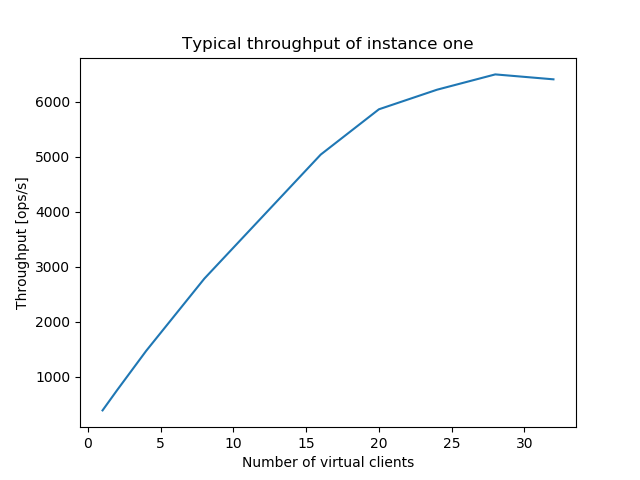
\includegraphics[width=\linewidth]{/home/simon/Documents/ETH/asl/asl-fall17-project/collectedStatFiles/Exp2/baseline2/readInst1Throughput.png}
\end{minipage}
\hfill
\begin{minipage}{0.5\linewidth}
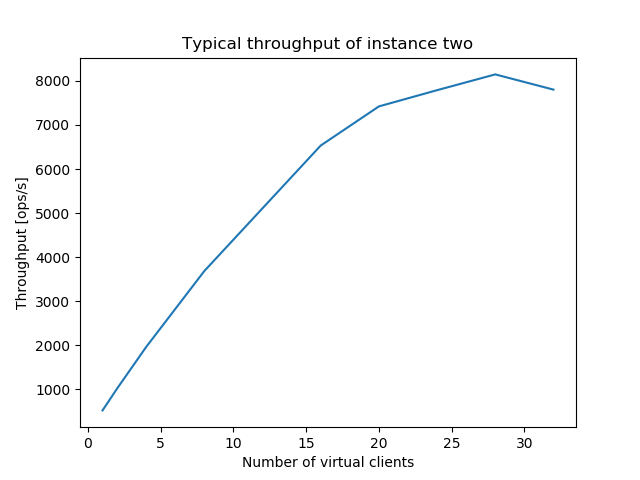
\includegraphics[width=\linewidth]{/home/simon/Documents/ETH/asl/asl-fall17-project/collectedStatFiles/Exp2/baseline2/readInst2Throughput.png}
\end{minipage}
\\\\
Remember that the client machine has two memtier instances each connected to a different memcached server. It is important to notice at this point that the maximal throughput achieved by the two instances are not equal. As shown on the next figures, this is because the latency is higher for one of the two servers, which may be because of their geographic location (The server located further away from the client machine results in a higher latency).
\begin{minipage}{0.5\linewidth}
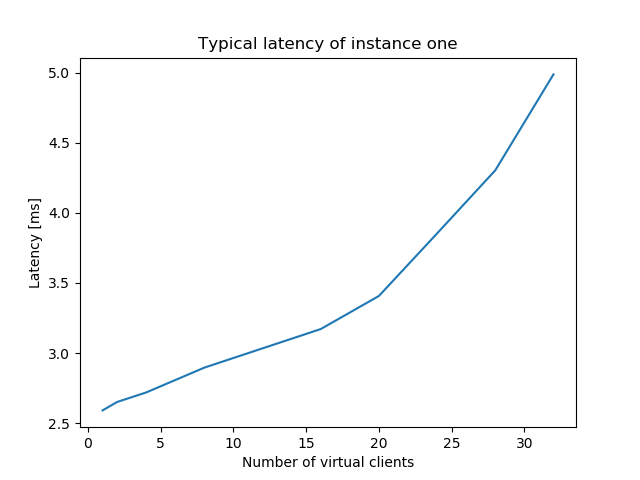
\includegraphics[width=\linewidth]{/home/simon/Documents/ETH/asl/asl-fall17-project/collectedStatFiles/Exp2/baseline2/readInst1Latency.png}
\end{minipage}
\hfill
\begin{minipage}{0.5\linewidth}
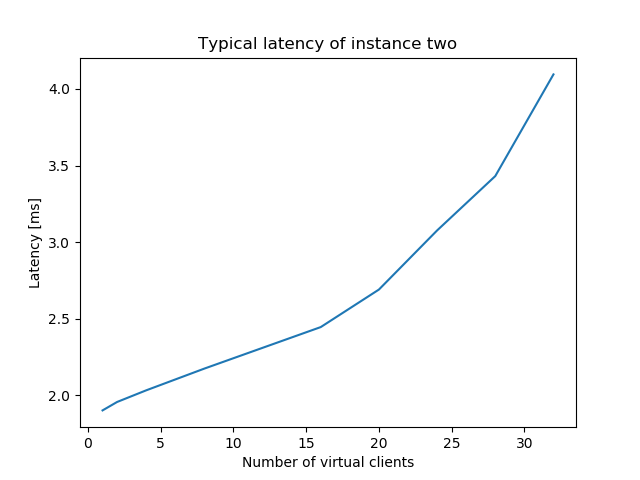
\includegraphics[width=\linewidth]{/home/simon/Documents/ETH/asl/asl-fall17-project/collectedStatFiles/Exp2/baseline2/readInst2Latency.png}
\end{minipage}
\\\\
For a write-only workload, we obtain for the server with higher throughput similar plots for throughput and latency than for a read-only workload:\footnote{exp2/baseline2/client01inst2\_ratio1:0\_rep1.txt}
\\
\begin{minipage}{0.5\linewidth}
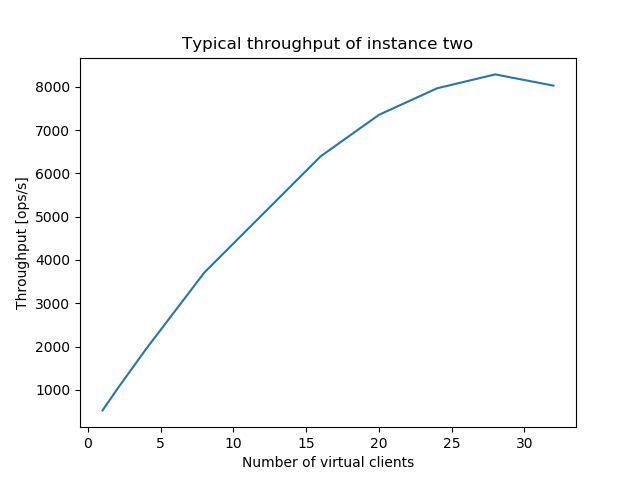
\includegraphics[width=\linewidth]{/home/simon/Documents/ETH/asl/asl-fall17-project/collectedStatFiles/Exp2/baseline2/writeInst2Throughput.png}
\end{minipage}
\hfill
\begin{minipage}{0.5\linewidth}
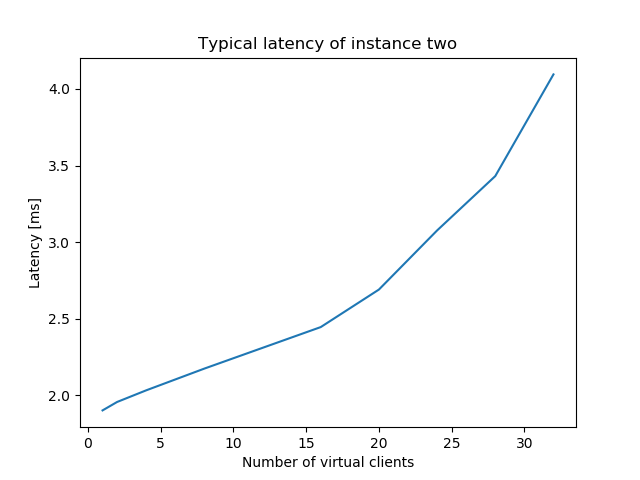
\includegraphics[width=\linewidth]{/home/simon/Documents/ETH/asl/asl-fall17-project/collectedStatFiles/Exp2/baseline2/writeInst2Latency.png}
\end{minipage}
\\
\\
We see that the system starts to saturate for the two workloads when reaching 28 virtual clients per thread, with a maximum throughput of around 8000 operations per second for the instance with higher throughput.  
We also note that contrary to the last experiment with a single server, the throughputs for write and read operations are similar. This proves for the last experiment that the memcached server saturates under a high read-only workload, but tends to be more scalable for write-only operations, since on the other hand, a single client machine cannot produce a higher throughput than 8000 operations per second, for reads nor for writes.   
\subsection{Summary}


Based on the experiments, we are now able to fill the table with the maximal throughputs for different configurations. To make the results suitable for comparison with the rest of the experiments, we sum up the throughputs observed on the different client machines for a single server. For the experiment with a single memtier client, we use the results of both instances to give a lower and upper bound (separated by a "/").\footnote{We used the same stats as for the last plots}

\begin{center}
	{Maximum throughput measured on one VM}
	\begin{tabular}{|l|p{2cm}|p{2cm}|p{4cm}|}
		\hline                        & Read-only workload & Write-only workload & Configuration gives max. throughput \\ 
		\hline One memcached server   &11289                    &23836                     &8 VC for read-only, 32  VC for write-only                                     \\ 
		\hline One load generating VM &6498/8146                    &6558/8287                     &28 VC                                     \\ 
		\hline 
	\end{tabular}
\end{center}
As explained in the previous sections, the key take-aways of this experiment are the following:

\begin{itemize}
\item The achieved throughput by the memtier clients may vary because of the geographic position of the clients or other factors. 
\item The memcached servers saturate faster for a read-only workload. For a write-only workload, the throughput can be twice as high and is limited by the performance of the memtier clients. 
\item We were able to find out the performance limitations of bothe a memtier client (line 2 of the table) and a memcached server (line 1). 
\end{itemize}
\newpage

\section{Baseline with Middleware}

In this set of experiments we want to take a closer look at the effect of the middleware on the system. For this purpose, we run experiments with different workloads, a different number of worker threads in the middleware, and one or two middlewares. This will show us in what way the middleware influences the results found during experiment 2. 


\subsection{One Middleware}

We start the experiment by connecting a single client machine to the middleware and one memcached server, for different workloads and number of worker threads: 

\begin{center}
	\scriptsize{
		\begin{tabular}{|l|c|}
			\hline Number of servers                & 1                        \\ 
			\hline Number of client machines        & 1                        \\ 
			\hline Instances of memtier per machine & 1                        \\ 
			\hline Threads per memtier instance     & 2                        \\
			\hline Virtual clients per thread       & [1..32]                  \\ 
			\hline Workload                         & Write-only and Read-only \\
			\hline Number of middlewares            & 1                        \\
			\hline Worker threads per middleware    & [8..64]                  \\
			\hline 
		\end{tabular}
	} 
\end{center}

\subsubsection{Results and explanation}

The throughput and the response time for a read-only workload measured on the middleware yield the following plots (the results for a write-only workload are similar):\footnote{files from exp3/normal, repetition 1, ratio 0:1}

\begin{center}
\includegraphics[scale=0.8]{/home/simon/Documents/ETH/asl/asl-fall17-project/collectedStatFiles/Exp3/part1/normal/statsMW/ratio0:1/rep1/throughput.png}
\end{center}
\begin{center}
\includegraphics[scale=0.8]{/home/simon/Documents/ETH/asl/asl-fall17-project/collectedStatFiles/Exp3/part1/normal/statsMW/ratio0:1/rep1/responseTime.png}
\end{center}

Note that the response time measured is the addition of the service time and the queuing time, as showed by the two following plots. 
\\
\begin{minipage}{0.5\linewidth}
\includegraphics[width=\linewidth]{/home/simon/Documents/ETH/asl/asl-fall17-project/collectedStatFiles/Exp3/part1/normal/statsMW/ratio0:1/rep1/serviceTime.png}
\end{minipage}
\hfill
\begin{minipage}{0.5\linewidth}
\includegraphics[width=\linewidth]{/home/simon/Documents/ETH/asl/asl-fall17-project/collectedStatFiles/Exp3/part1/normal/statsMW/ratio0:1/rep1/timeInQueue.png}
\end{minipage}
\\
By taking a close look at the statistics\footnote{any file in experience 3 can be considered for this point}, we observe that the service time is essentially the time apent waiting for an answer from the mmecached server. Since the service time is defined as \(serviceTime = parsingTime + waitingForMemcached\), and that we see that the parsing time is very small, the service time is essentially the time waiting for an answer. 
\\
The interactive law is also respected: if we take for example 16 middleware worker threads and 32 virtual clients, we obtain \(N = 64, X = 6000,\) and thus \(w = 10 ms\), which is not far from what we plotted (in reality, as we will see later, the time spent in the middleware, known as "think time" has also to be taken into account). 
\\
From the four of these previous plots, we see that the middleware is the bottleneck for a configuration with 8 and 16 middleware worker threads, since the throughput stays constant after respectively 8 and 16 virtual client and, as seen in the last experiment, the maximum throughput that can be achieved by memtier is higher than the throughputs achieved here. More precisely, the bottleneck in the middleware is the time a request spends in the queue, as shown by the strongly increasing curve of the average time in queue for 8 worker threads for example, which can be up to 5 times as big as the service time. This strong growth of the queuing time is also correlated to the average queue length: as shown in the next figure, the queue length is growing with the time a request spends in queue, since the middleware has not enough threads available to execute the requests. 
\begin{center}
\includegraphics[scale=0.5]{/home/simon/Documents/ETH/asl/asl-fall17-project/collectedStatFiles/Exp3/part1/normal/statsMW/ratio0:1/rep1/queueLength.png}
\end{center}
As a sanity check, we also plot the latency and the throughput observed on the client:
\\
\begin{minipage}{0.5\linewidth}
\includegraphics[width=\linewidth]{/home/simon/Documents/ETH/asl/asl-fall17-project/collectedStatFiles/Exp3/part1/normal/statsClient/ratio0:1/rep1/throughput.png}
\end{minipage}
\hfill
\begin{minipage}{0.5\linewidth}
\includegraphics[width=\linewidth]{/home/simon/Documents/ETH/asl/asl-fall17-project/collectedStatFiles/Exp3/part1/normal/statsClient/ratio0:1/rep1/latency.png}
\end{minipage}
\\
There are two interesting points to notice: first, the throughput measured on the middleware is equal to the one measured on the memtier VM, which is due to the way memtier works. As explained in section 1, one memtier CPM doesn't send a new request until the last one has not been received. Secondly, the graph of the latency is similar in shape as the one for the response time on the middleware, but shifted by 2ms on the y-axis, which is due to the travelling time between the middleware and the memtier client. 
\\
\\
As a last point, because we haven't reached a saturated middleware with 32 and 64 worker threads, we re-run the experiment with an increased number of generating client VM (2), to obtain the following results for a read-only as well as for a write-only workload:\footnote{files from exp3/part1/bs, repetition 1, ratio 0:1}
\\
\begin{minipage}{0.48\linewidth}
\includegraphics[width=\linewidth]{/home/simon/Documents/ETH/asl/asl-fall17-project/collectedStatFiles/Exp3/part1/bs/statsMWBottSearch/throughput.png}
\end{minipage}
\hfill
\begin{minipage}{0.48\linewidth}
\includegraphics[width=\linewidth]{/home/simon/Documents/ETH/asl/asl-fall17-project/collectedStatFiles/Exp3/part1/bs/statsMWBottSearch/timeInQueue.png}
\end{minipage}
\\\\
The graphs above show that by increasing the workload, we are able to saturate the middleware with 32 worker threads, again, due to a slope change in the queuing time. For 64 worker threads, we tend to reach a saturated state at around 11000 operations per second, which also corresponds to the maximum throughput a memcached server can achieve with a read-only workload. To make sure that it is the middleware that becomes the bottleneck under high workload even with 64 worker threads, we have run all this experiment with a write-only workload also, and obtained for every configuration and every statistics the same plots. Seeing that the maximum throughput of the memcached server under a write-only workload was around 20000 ops/second, we can conclude that the middleware will start to become the bottleneck under any configuration if the throughput is high enough. 
   
\subsection{Two Middlewares}

We continue the experiment by connecting one client VM with two instances of memtier to two different middlewares VMs and one memcached server:

\begin{center}
	\scriptsize{
		\begin{tabular}{|l|c|}
			\hline Number of servers                & 1                        \\ 
			\hline Number of client machines        & 1                        \\ 
			\hline Instances of memtier per machine & 2                        \\ 
			\hline Threads per memtier instance     & 1                        \\
			\hline Virtual clients per thread       & [1..32]                  \\ 
			\hline Workload                         & Write-only and Read-only \\
			\hline Number of middlewares            & 2                        \\
			\hline Worker threads per middleware    & [8..64]                  \\
			\hline 
		\end{tabular}
	} 
\end{center}
\subsubsection{Results and explanation}

We obtain the following plots for the throughput and response time measured on one middleware with similar plots for read-only and write-only workloads:\footnote{files from exp3/part2/normal, repetition 1, ratio 0:1}
\\
\begin{minipage}{0.42\linewidth}
\includegraphics[width=\linewidth]{/home/simon/Documents/ETH/asl/asl-fall17-project/collectedStatFiles/Exp3/part2/normal/mw1/throughput.png}
\end{minipage}
\hfill
\begin{minipage}{0.42\linewidth}
\includegraphics[width=\linewidth]{/home/simon/Documents/ETH/asl/asl-fall17-project/collectedStatFiles/Exp3/part2/normal/mw1/responseTime.png}
\end{minipage}
\\
We directly notice that the difference of throughput and reponse time between different numbers of worker threads configuration isn't as significant as during the last experiment. As we will see on the next plots, this is because the high queuing time for a lower number of worker threads is compensated by a low service time and inversely. 
\\
\begin{minipage}{0.49\linewidth}
\includegraphics[width=\linewidth]{/home/simon/Documents/ETH/asl/asl-fall17-project/collectedStatFiles/Exp3/part2/normal/mw1/serviceTime.png}
\end{minipage}
\hfill
\begin{minipage}{0.49\linewidth}
\includegraphics[width=\linewidth]{/home/simon/Documents/ETH/asl/asl-fall17-project/collectedStatFiles/Exp3/part2/normal/mw1/timeInQueue.png}
\end{minipage}
\\\\ 
We should also take into consideration that the workload exerced on one middleware is halved compared to the last experiment , where there was only one thread per memtier instance and not two, which explains why the average time in queue for 8 worker threads only starts to grow faster after 16 virtual clients as opposed to 8 virtual clients. Furthermore, the throughput at saturation for 8 middleware threads is equal to the last experiment. 
Deducing from the previous experiment where we learnt that the bottleneck in the middleware is the queuing time, and the graphs above, the middleware hasn't reached its maximal throughput for the other configurations. 
\\\\
However, when we double the load on the middlewares, we can see that our middleware isn't the bottleneck of the experiment if we put a high number of worker thread, but the memcached server. To prove this claim, we remember from the conclusions of Section 2 that the memcached server achieves a higher throughput with a write-only workload than a read-only. However, as shown in the last experiment, the throughput achieved through a middleware with the two workloads is equal, given the middleware is the bottleneck. The two following plots show that even if the throughputs start to flatten out the two workloads lead to a \underline{different} throughput\footnote{files from exp3/part2/bs/mw1, repetition 2, ratio 0:1 and 1:0}   
\\
\begin{minipage}{0.5\linewidth}
\includegraphics[width=\linewidth]{/home/simon/Documents/ETH/asl/asl-fall17-project/collectedStatFiles/Exp3/part2/bs/statsMW01BottleneckSearch/ratio0/throughput.png}
\end{minipage}
\hfill
\begin{minipage}{0.5\linewidth}
\includegraphics[width=\linewidth]{/home/simon/Documents/ETH/asl/asl-fall17-project/collectedStatFiles/Exp3/part2/bs/statsMW01BottleneckSearch/ratio1/throughput.png}
\end{minipage}
\\\\
To confirm our claim further, the calculation of the total throughput through the two middlewares on a single memcached server for read and write-only are:
\\\textit{read : 4173+7043 = 11216 operations/second}
\\\textit{write : 5452+10753 = 16205 operations/second}
\\
Hence, because the maximum throughput of a single memcached server for read-only workload was 11289, and 23836 for write-only, this proves that the memcached server is the bottleneck for this further experiment for a read-only workload. In other words, we can reach the memcached server upper-bound with a configuration with 64 worker thread and 2 connected middlewares for read-only. 



\subsection{Summary}
The maximum throughputs for different configurations are summarized in the following table. The throughputs are added over all the VM as well for the middlewares than the clients.\footnote{files from exp3, part 1 or 2, bs: all with 64 mwt, repetition1} 

\begin{center}
	{Maximum throughput for one middleware.}
	\begin{tabular}{|l|p{2cm}|p{2cm}|p{2cm}|p{2cm}|}
		\hline                                & Throughput& Response time[ms] & Average time in queue[ms] & Miss rate \\ 
		\hline Reads: Measured on middleware  &10638           &6.69              &2.07                       &14\%           \\ 
		\hline Reads: Measured on clients     &10266            &12.25               &-                  &14\%           \\ 
		\hline Writes: Measured on middleware &10477            &7.17               &2.13                       &-      \\ 
		\hline Writes: Measured on clients    &10128            &12.63               &-                  &-       \\ 
		\hline 
	\end{tabular}
\end{center}

For this experiment, we take the average of the times since both middlewares don't have the same throughput. 
\begin{center}
	{Maximum throughput for two middlewares.}
	\begin{tabular}{|l|p{2cm}|p{2cm}|p{2cm}|p{2cm}|}
		\hline                                & Throughput & Response time & Average time in queue & Miss rate \\ 
		\hline Reads: Measured on middleware  &11216            &10.21               &1.09                       &0.1\%           \\
		\hline Reads: Measured on clients     & 11618            &12.246               &-                   &0.1\%           \\ 
		\hline Writes: Measured on middleware &16205            &6.305               &0.93                       &-       \\ 
		\hline Writes: Measured on clients    &16019            &8.915               &-                   &-       \\ 
		\hline 
	\end{tabular}
\end{center}

As explained in the previous sections, the key take-aways for this experiment are the followings:

\begin{itemize}
\item The bottleneck of the middleware is the queuing time of the requests. When the number of worker threads is too low, this value tends to grow very fast.  
\item The same observation applies for a configuration with two middlewares. If the performance of the memcached servers and memtier benchmark clients were infinitely good, we would expect a performance twice as high than for one middleware, since they run independently. But this is not the case and could show that we can achieve the upper-bound of the memcached server with two middlewares and a read-only workload. 
\end{itemize}
\newpage

\section{Throughput for Writes}

\subsection{Full System}

The purpose of this section is to assess the behaviour of the middleware with a write-only workload and increased number of clients and servers.

\begin{center}
	\scriptsize{
		\begin{tabular}{|l|c|}
			\hline Number of servers                & 3          \\ 
			\hline Number of client machines        & 3          \\ 
			\hline Instances of memtier per machine & 2          \\ 
			\hline Threads per memtier instance     & 1          \\
			\hline Virtual clients per thread       & [1..32]    \\ 
			\hline Workload                         & Write-only \\
			\hline Number of middlewares            & 2          \\
			\hline Worker threads per middleware    & [8..64]    \\
			\hline 
		\end{tabular}
	} 
\end{center}

\subsubsection{Results and explanation}

The statistics of a single middleware have as expected the same shape than during last experiment, and are nearly equal between two middlewares. Hence, we plot here the total throughput of the two middlewares and the other statistics from one single middleware.\footnote{files from exp4, mw1 and 2, repetition 2} 

\begin{center}
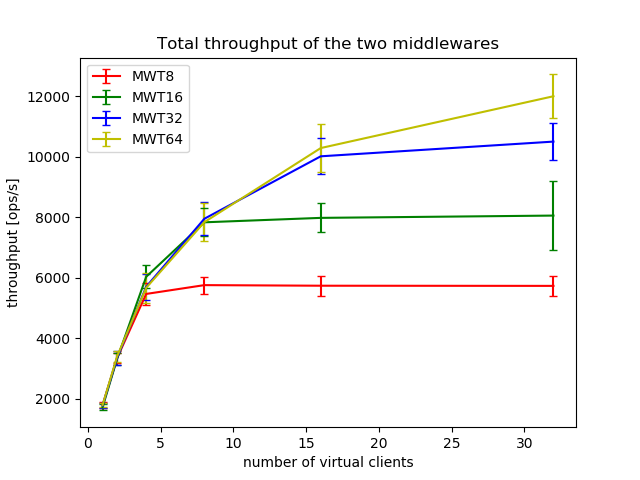
\includegraphics[scale=0.57]{/home/simon/Documents/ETH/asl/asl-fall17-project/collectedStatFiles/Exp4/totalThroughputM1and2/totalThroughput.png}
\end{center}
 \begin{center}
\includegraphics[scale=0.57]{/home/simon/Documents/ETH/asl/asl-fall17-project/collectedStatFiles/Exp4/statsMW1/responseTime.png}
\end{center}

The interactive law also holds for this case. If we take for example 32 worker threads at 16 virtual clients, we get \(N = 16\) $\cdot$ 6 (since there are 3 clients putting workloads on these two middleware), \(X = 10000\), yields \(w = 0.0096 = 9.6 ms\), which is approximately correct when we compare it with the graph. 
We further notice that the latency takes much higher values than during the last experiment, which is due to an increased workload from more clients. 
\\
We now want to get an insight on the service time compared to the queuing time.
\\
\begin{minipage}{0.5\linewidth}
\includegraphics[width=\linewidth]{/home/simon/Documents/ETH/asl/asl-fall17-project/collectedStatFiles/Exp4/statsMW1/serviceTime.png}
\end{minipage}
\hfill
\begin{minipage}{0.5\linewidth}
\includegraphics[width=\linewidth]{/home/simon/Documents/ETH/asl/asl-fall17-project/collectedStatFiles/Exp4/statsMW1/timeInQueue.png}
\end{minipage}
\\\\
We notice that the service time stays constant after reaching a certain threshold. As we can see on the graph on the right, this is because of the time a request spends in queue. At one point, too many requests enter the middleware and can't be processed directly due to the number of available worker threads. We also see that the service time is higher for an increased number of middleware threads, which is due to the workload  put on the memcached server. For a low number of worker threads, the service time stays low due to an under-saturated memcached server. 
A tradeoff between service time and average queuing is also to be seen: A higher number of worker threads will increase the load on the memcached server and its response time, whereas a too low number of middleware threads skyrockets the queuing time. This is why the gap between the response times (single graph above for response) is big for a low number of middleware threads and grows smaller when increasing the number of worker threads. 
\\
At last, we have a look at the average queue length in the middleware:
\begin{center}
\includegraphics[scale=0.5]{/home/simon/Documents/ETH/asl/asl-fall17-project/collectedStatFiles/Exp4/statsMW1/queueLength.png}
\end{center}
As said in the previous experiment, the average queue length follows the shape of the queuing time. A small calulation allows us to explain these numbers. 
If we consider our middleware with \textit{m} number of worker threads, an average queue length of \textit{L}, the service time being \textit{s}, and the waiting time in queue being \textit{T}, we can verify that: 
\[ T = \frac{L}{m}\cdot s \]
which is just the number of requests awaiting for a given worker thread times the average service time of one worker thread. For example, if we take m = 16 and the number of virtual clients 32, we have L = 65, s = 4ms, and thus we obtain T = 16.25ms, which corresponds to what we measured (when looking at the previous graphs)
\subsection{Summary}
To fill in the summary table, we calculate the total throughput of the middlewares, and take one representative statistic for the rest. For the throughput derived from the MW response time we use the interactive law as showed at the start of this section.\footnote{We use all the files of experiment 4, repetition 2} 
\begin{center}
	{Maximum throughput for the full system}
	\begin{tabular}{|l|p{1.5cm}|p{1.5cm}|p{1.5cm}|p{1.5cm}|}
		\hline                                            & WT=8 & WT=16 & WT=32 & WT=64 \\ 
		\hline Throughput (Middleware)                    &5734      &8060       &10507       &12008       \\ 
		\hline Throughput (Derived from MW response time) &5485      &9142       &12000       &14906       \\ 
		\hline Throughput (Client)                        &5769      &8438       &10384       &11791       \\ 
		\hline Average time in queue[ms]                      &31.2      &18.3       &10.0      &3.4       \\ 
		\hline Average length of queue                    &84      &72       &47       &19       \\ 
		\hline Average time waiting for memcached[ms]         &2.9      &3.9       &6.1       &9.3       \\ 
		\hline 
	\end{tabular}
\end{center}

The key take-aways for this experiment are the following: 
\begin{itemize}
\item There exists a tradeoff between the queuing time and the time waiting for memcached: The higher the number of worker threads, the higher the load on the memcached servers, but the lower the queuing time becomes and inversely
\item We could apply a simple law that links the service time, the number of worker threads, the length of the queue and the queuing time, as well as the interactive law. 
\end{itemize}
\newpage

\section{Gets and Multi-gets}

In this set of experiments we will have a closer look at the behaviour of the system with get and multi-get requests. First, at the sharded case, where the middleware splits the requests among the servers, and secondly at the non-sharded case, where the request is handled as a normal get. 

\subsection{Sharded Case}
The memtier workload is adapted so that memtier sends one set request alternated with one multi get request of the key-size we want. Also, we use 64 middleware threads to achieve maximum throughput. 

\begin{center}
	\scriptsize{
		\begin{tabular}{|l|c|}
			\hline Number of servers                & 3                       \\ 
			\hline Number of client machines        & 3                       \\ 
			\hline Instances of memtier per machine & 2                       \\ 
			\hline Threads per memtier instance     & 1                       \\
			\hline Virtual clients per thread       & 2     		            \\ 
			\hline Workload                         & [1:1, 1:3, 1:6, 1:9]           \\
			\hline Multi-Get behavior               & Sharded                \\
			\hline Multi-Get size                   & [1, 3, 6, 9]                  \\
			\hline Number of middlewares            & 2                       \\
			\hline Worker threads per middleware    & 64 \\
			\hline 
		\end{tabular}
	} 
\end{center}

\subsubsection{Results and explanations}
First, we analyze a couple of statistics on the middleware to understand its behaviour. The throughput and the service time on one middleware are plotted:\footnote{files from exp5, mw1, repetition1 (through the whole part)}
\\
\begin{minipage}{0.5\linewidth}
\includegraphics[width=\linewidth]{/home/simon/Documents/ETH/asl/asl-fall17-project/collectedStatFiles/Exp5/statsMW1//shardedtrue/serviceTime.png}
\end{minipage}
\hfill
\begin{minipage}{0.5\linewidth}
\includegraphics[width=\linewidth]{/home/simon/Documents/ETH/asl/asl-fall17-project/collectedStatFiles/Exp5/statsMW1//shardedtrue/throughput.png}
\end{minipage}
\\\\
We observe that the service time increases with the key size, which is normal since the processing the middleware has to do for different key sizes is approximately equivalent, but the time taken by the server to process the request and send the packet back is higher for a bigger key amount. For the sharded case, we know that the middleware has to split the requests into different servers, which may cause a bigger processing time. However, this additional processing time can be neglected as shown by the following graphics (the left one represents the total time a request spends in the multi get handling, whereas the right graphic shows the waiting time for memcached in the multi get handling). In fact the differences between the two is in micro seconds. 
\\
\begin{minipage}{0.5\linewidth}
\includegraphics[width=\linewidth]{/home/simon/Documents/ETH/asl/asl-fall17-project/collectedStatFiles/Exp5/statsMW1//shardedtrue/timesInMGet.png}
\end{minipage}
\hfill
\begin{minipage}{0.5\linewidth}
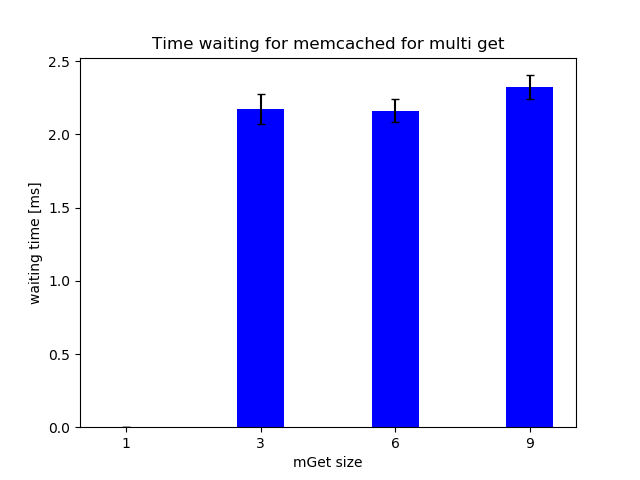
\includegraphics[width=\linewidth]{/home/simon/Documents/ETH/asl/asl-fall17-project/collectedStatFiles/Exp5/statsMW1//shardedtrue/timesInMGetMem.png}
\end{minipage}
\\\\
Two comments have to be made regarding these graphs: first, we see that there is no statistic for a key size of 1, which is because a multi get with size one is handled as a get in the middleware and thus isn't part of the multi get statistics. Secondly, we observe that the time spent in the multi get handling is equivalent to the service time. This is because the parsing time of a request is still very small even if the size of the message grows.
\\
In the previous sections, we discovered that the time spent in the queue was the bottleneck of our system. However, in a multi get configuration, this isn't the case any more as shown by the following figure, which plots the time spent in queue:  
 \begin{center}
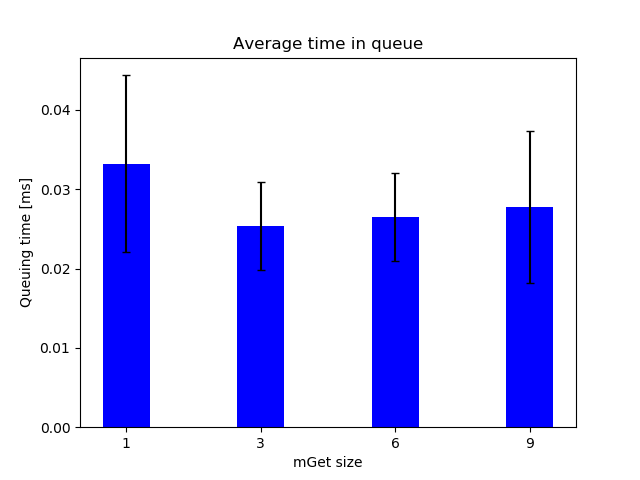
\includegraphics[scale=0.6]{/home/simon/Documents/ETH/asl/asl-fall17-project/collectedStatFiles/Exp5/statsMW1//shardedtrue/timesInQueue.png}
\end{center}


On the client side, a closer look is taken at the latency distribution of the requests. The plotted line represents the average latency. The colors represent the percentage of the requests that are in a certain latency range. Thus, the top ends of the color bars represent respectively the 25th, 50th, 75th, 90th and 99th percentiles.\footnote{files exp5, client1, repetition 1} 
  
 \begin{center}
\includegraphics[scale=0.7]{/home/simon/Documents/ETH/asl/asl-fall17-project/collectedStatFiles/Exp5/statsClient1//shardedTrue/latency.png}
\end{center}

We observe a similar behaviour than on the middleware with a small growth of the latency and that the values are clustered around the average as expected. A closer look at the distribution of the latency will be made at the end of this section. 

\subsection{Non-sharded Case}

The middleware is now run in non-sharded mode. A multi-get request is therefore handled in the same way as a normal get. 

\begin{center}
	\scriptsize{
		\begin{tabular}{|l|c|}
			\hline Number of servers                & 3                       \\ 
			\hline Number of client machines        & 3                       \\ 
			\hline Instances of memtier per machine & 2                       \\ 
			\hline Threads per memtier instance     & 1                       \\
			\hline Virtual clients per thread       & 2                		 \\ 
			\hline Workload                         & [1:1, 1:3, 1:6, 1:9]             \\
			\hline Multi-Get behavior               & Non-Sharded             \\
			\hline Multi-Get size                   & [1..9]                  \\
			\hline Number of middlewares            & 2                       \\
			\hline Worker threads per middleware    & 64 \\
			\hline 
		\end{tabular}
	} 
\end{center}

\subsubsection{Results and explanation}

The results are extremely similar to the sharded case: we observe a growth of the latency with the number of keys in the multi get. The latency as observed on the middleware and on the clients are shown as followed: 
\\
\begin{minipage}{0.5\linewidth}
\includegraphics[width=\linewidth]{/home/simon/Documents/ETH/asl/asl-fall17-project/collectedStatFiles/Exp5/statsMW1//shardedfalse/timesInMGet.png}
\end{minipage}
\hfill
\begin{minipage}{0.5\linewidth}
\includegraphics[width=\linewidth]{/home/simon/Documents/ETH/asl/asl-fall17-project/collectedStatFiles/Exp5/statsClient1/shardedFalse/latency.png}
\end{minipage}
\\\\
For this part, there is no surprise regarding the obtained results. As the key size grows, the memcached server needs more time to process the request and send the answer back, and thus we observe a growth of the latency. A detailed comparison between the sharded and non sharded case can be found in the two next sections. 

\subsection{Histogram}

The distribution of the latency as measured on the middleware and the client, for both sharded and non sharded case, for a key size of 6, yields the following plots (the histograms are constructed in a way so that bins having less than one request are not displayed):
\\
\begin{minipage}{0.5\linewidth}
\includegraphics[width=\linewidth]{/home/simon/Documents/ETH/asl/asl-fall17-project/collectedStatFiles/Exp5/statsClient1/shardedTrue/histogram6.png}
\end{minipage}
\hfill
\begin{minipage}{0.5\linewidth}
\includegraphics[width=\linewidth]{/home/simon/Documents/ETH/asl/asl-fall17-project/collectedStatFiles/Exp5/statsMW1/shardedtrue/HistMGetsize6.png}
\end{minipage}
\\
\\
\begin{minipage}{0.5\linewidth}
\includegraphics[width=\linewidth]{/home/simon/Documents/ETH/asl/asl-fall17-project/collectedStatFiles/Exp5/statsClient1/shardedFalse/histogram6.png}
\end{minipage}
\hfill
\begin{minipage}{0.5\linewidth}
\includegraphics[width=\linewidth]{/home/simon/Documents/ETH/asl/asl-fall17-project/collectedStatFiles/Exp5/statsMW1/shardedfalse/HistMGetsize6.png}
\end{minipage}


\subsection{Summary}

All the histograms seem to follow a gaussian distribution around a shifted mean. First, we notice that the measured response time on the client is slightly higher than the one measured on the middleware, due to the travelling time between the middleware and the client. Secondly, more interesting, the latency is on average higher in the sharded case than in the non sharded case. 
\\
This can be explained by the following points: 
\begin{itemize}
\item The server performance is similar if it receives 2 keys in the get requests (in the sharded case with 3 servers) or 6 keys. This claim can be proved by looking at the graph in section 5.2, where we see that the difference of time spent in the multi get handling between 3 and 6 keys , i.e the difference of waiting time for the memcached server, is very small. Hence, reducing the key size from 6 to 2 isn't enough to observe a significant difference in latency. 
With a multi get key size of 9, the difference wouldn't have been significant either, by refering to the same graph, since the request would have been split in sizes of 3. A major difference could have been observed if we had a key size of n which overwhelms the server, whereas a size of n/3 doesn't. However, n=9 isn't enough to overwhelm the server, even with a very low miss ratio (1\%)
\item The way the middleware handles a multi-get request in the sharded mode isn't optimal. The pattern followed by the multi get handling is the same as the one for a set request, namely: 
\begin{lstlisting}
	1				prepare the splitted requests
	2				send to server 1
	3				send to server 2
	4				send to server 3
	5				wait for answer 1 until received
	6				wait for answer 2 until received
	7				wait for answer 3 until received
	8				merge the answers and send back to client
\end{lstlisting}
Like we discussed in Section 1, the point 1 is extremely efficient and can be neglected. However, waiting sequentially for an answer from a server can be bad if the response times are different as explained for set requests. 
\end{itemize}  

\newpage
\section{2K Analysis}
In this section we perform a 2k analysis with 3 parameters and 3 repetitions. We want to analyze the explained variation of the number of servers, the number of worker threads and the number of middlewares. 
\subsection{Parameters of the experiment}
The following configuration are beeing experimented:
\begin{center}
	\scriptsize{
		\begin{tabular}{|l|c|}
			\hline Number of servers                & \textbf{2 and 3}                                     \\ 
			\hline Number of client machines        & 3                                           \\ 
			\hline Instances of memtier per machine & 2                                           \\ 
			\hline Threads per memtier instance     & 1                                           \\
			\hline Virtual clients per thread       & 32                                     \\ 
			\hline Workload                         & Write-only, Read-only, and 50-50-read-write \\
			\hline Number of middlewares            & \textbf{1 and 2}                                     \\
			\hline Worker threads per middleware    & \textbf{8 and 32}                                    \\
			\hline 
		\end{tabular}
	} 
\end{center}
\subsection{Results and explanation}
The full calculations for this 2\textsuperscript{3}\(\cdot\)3 analysis can be found in the excel sheet called \textit{SummaryStats.ods}. The final results obtained for a 2k analysis for the throughput are displayed here:
\begin{center} 
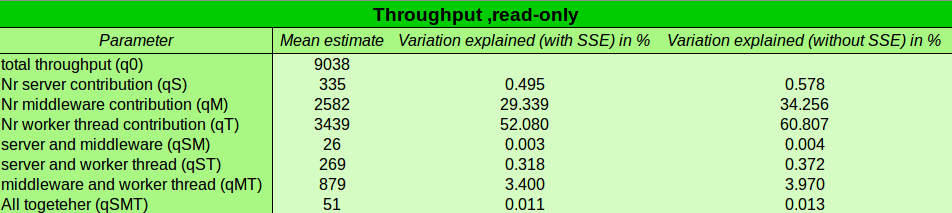
\includegraphics[width=\linewidth]{/home/simon/Documents/ETH/asl/asl-fall17-project/collectedStatFiles/Exp6/tro.png}
\end{center}
The obtained results are as expected, not a surprise, and only confirm what we concluded from the last experiments.
\\
For the throughput, the contribution of the variation of the number of servers is very low. As it could be seen during the last experiments, the time spent in queue in the middleware has always been the bottleneck of our system when using a single get workload. In addition, as observed in experiment 5, using more servers doesn't improve the total time waiting for the memcached server(s), and thus, changing the number of servers only explains few variation. 
\\
The explained variation is basically shared between the single contribution of the increase of the number of middlewares, and the single contribution of the increase of the numer of worker threads. This point has also been highlighted in the previous experiments: the throughput increases drastically with the number of worker threads, and only increases up to a certain point with two middlewares because of the memcached server capacity. That's why the variation explained by the number of worker threads is twice as high than the variation explained by the number of middlewares. This is a further proof that the times in queue is the biggest bottleneck in our system, and that changing its value influences a lot on the throughput. 
\\We finally note that the different factors of this experiment are quite independent since their combined values are very low. 
\newpage

For the response time, the 2k analysis leads to the following results:
\\
\begin{center} 
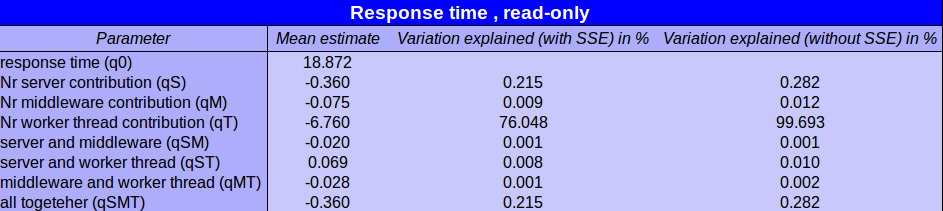
\includegraphics[width=\linewidth]{/home/simon/Documents/ETH/asl/asl-fall17-project/collectedStatFiles/Exp6/rro.png}
\end{center} 
For the response time, we note that the contributions are all negative. This is, because of the fact that if we increase a factor (for example from 8 worker threads to 32), we decrease the response time. 
\\
For the reponse time, only the variation of the number of middleware threads has a significant influence on the response time. The number of servers has (nearly) no influence on the response time, for the same reason that it didn't have for the throughput. On the other hand, the number of middleware has also no influence on the response time, because the response time on two middlewares are independent of each other as long as the memcached servers (which are the same for the two middlewares) are not saturated, which is not the case as we can observe in this table. In the case where the servers would be oversaturated, we would have a positive contribution for qM. 
\\Finally, the number of worker threads is again the main contributor to the variation of the response time. For the same reasons as for the troughput, a higher number of worker threads leads to a lower queuing time and thus a faster response time. 
\\\\
The response time and the throughput tables for the other workloads are very similar and are not treated in this report (but can be found in the \textit{SummaryStats.ods} file), since the same comments apply to them. 
\newpage
\section{Queuing Model}
So far, statistics have been collected, plotted and analyzed. We now want to model our system to be able to predict these different statistics. The statistics that we calculate and compare with the statistics collected on a single middleware are taken from the book \textit{The Art of computer systems performance analysis by Raj Jain}, pages 532 and 536. 

\subsection{M/M/1}

To model our system as a M/M/1 model, the statistics collected from experiment 4 are used. 
The M/M/1 model is a basic modelling system that models one queue with exponentially distributed  service times and arrival rate (the two "M"), and one "server". In our case, this means that the M/M/1 model represents a system where the requests arrive on one unique queue and are being processed by a "single-processor" system, i.e one unique thread that takes and processes the requests from the queue.
\\
To be able to model our system as a M/M/1 model, we need to tweak the results somehow to make it appropriate to be used to calculate the statistics. In our middleware, we computed the mean service time that a worker thread takes to process a request, which is (as can be seen in any stat files, by comparing the individual service time per thread and the mean service time) representative of the service time of a single worker thread. Assuming that this mean service time is the service time of the "single-processor" is incorrect: it leads to assume that one request is handled during the average service time of a worker thread. In fact, if the number of worker threads on the middleware is \textit{mwt}, approximately \textit{mwt} requests are  handled during this time-lapse, since they are run in parallel! (since we are able to assume that context switching and other artifacts can be neglected). In consequence, the service time that we are using to calculate these statistics is: 
\[\frac{service Time}{mwt}\]
\\
To build a M/M/1 queuing model, the traffic intensity is beeing computed, which is the ratio between the arrival rate and the service rate. If this ratio is smaller than 1, the system is said to be "stable", otherwise it is "unstable". In our case, having a ratio bigger than 1 means that the middleware is saturated, i.e too many requests are coming in than what can be processed, and a ratio of 1 is beeing obtained, when the throughput starts to flatten out. As we discussed in the \textit{System overview} section, a ratio bigger than 1 is nearly impossible to achieve because memtier won't send more requests than what it receives back. However, small errors linked to statistics gathering can lead to having a ratio slightly over 1, even if it should be a little bit less than 1 in reality. For this reason, we will not be able to analyze the system when the ratio is getting close to 1, as the system will be described as "unstable".
\\\\
We start by computing the different statistics for a middleware configuration with 8 threads for 2 virtual clients\footnote{files from exp4, mw1, repetition 1, throughout the section} , which gives an arrival rate of 1568 requests/sec and a service time of 2813709ns per thread. As discussed previously, we use 2813709/8 = 351713ns as an input for the service time. The output from these calulations are found on the first line, the statistics collected from the middleware on the second line:\footnote{P0: probability of having 0 jobs in the system\\P1/P2: probability of having 1 respecitvely two jobs in the system}: 
\begin{center}

		\begin{tabular}{|c|c|c|c|c|c|}
			  \hline
			  \textbf{P0} & \textbf{P1/P2} & \textbf{Jobs in system} & \textbf{Jobs in queue} & \textbf{response time[ms]} & \textbf{time in queue[ms]}\\
			  \hline
			  0.44 & 0.25/0.14 & 1.22 & 0.67 & 0.61 & 0.43 \\
			  - & - & - & 0.98  & 2.92 & 0.11 \\
			  \hline
		\end{tabular}
 
\end{center}
When comparing to the statistics, we see that the number of jobs in the system and number of jobs in the queue correspond. For the number of jobs in the system, since we modelled the system as an M/M/1 model, with the service time being \textit{serviceTime/mwt}, the number of jobs in the system will be 1.22$\cdot$\textit{mwt} in reality, which better corresponds to what we have in this configuration. 
 \\
However, the time spent in the queue doesn't correspond at all to what we measured on our middleware. This is because our system can simply not be modelled correctly with a M/M/1 model: In this model, it is assumed that a "single server", i.e a single thread is handling the incoming requests. Assuming that \textit{mwt} requests are handled in a time period T (multiple threads) is the same as one request is being handled in \textit{T/mwt} time (single thread) is not enough to model our system as an M/M/1. This is because multiple threads take requests from the queue in a round-robin fashion, whereas the single thread model takes one request at a time, executes it completely before taking another request. 

  
\subsection{M/M/m}

To model our system as a M/M/m model, the experiment 4 statistics are used again.
The M/M/m model has the same interarrival properties and queuing properties than the M/M/1 model. The only and crucial difference is that multiple "servers" are handling the requests being queued. In our case, multiple threads are handling the requests. A priori, this modelling seems to represent our system much better. We will see if this claim can be verified. 
\\
First of all, the same comment about the stability of the system applies to the M/M/m model: A ratio between the arrival rate and the service rate multiplied by the number of worker threads being bigger than 1 leads to an unstable system and the statistics cannot be computed. We compute the statistics with the same configuration as before, 8 worker threads, 1568 request/seconds for the arrival rate, and 2813709ns for the service time:

\begin{center}

		\begin{tabular}{|c|c|c|c|c|c|}
			  \hline
			  \textbf{P0} & \textbf{Jobs in system} & \textbf{Jobs in queue} & \textbf{response time[ms]} & \textbf{time in queue[ms]}\\
			  \hline
			  0.012  & 4.41 & 0.23 & 2.82 & 0.07 \\
			   - & - & 0.98  & 2.92 & 0.11 \\
			  \hline
		\end{tabular}
 
\end{center}
The probability distribution of the number of jobs in the system is plotted on the following chart: 
\begin{center} 
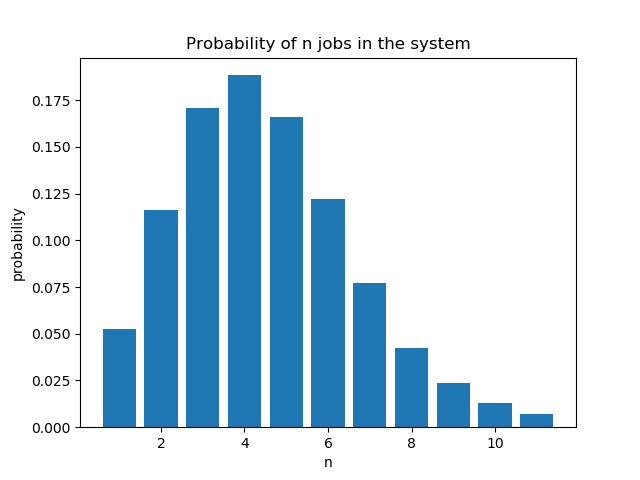
\includegraphics[scale=0.53]{/home/simon/Documents/ETH/asl/asl-fall17-project/Scripts/exp7/nJobsInSystem1.png}
\end{center} 
For the M/M/m model, the response time and the queuing time are predicted right, with a very small queuing time and a response time. The mean number of jobs in the queue also corresponds to the gathered statistics. However, it seems with the chart that the system is underused, with a probability of only 5-6\% that all the worker threads are in use. We want to verifiy this claim by taking a higher arrival rate with the same configuration, i.e 4 virtual clients, which yields an arrival rate of 2513 requests/second and a service time of 3036419ns. 
This leads to the following values:
 \begin{center}

		\begin{tabular}{|c|c|c|c|c|c|}
			  \hline
			  \textbf{P0} & \textbf{Jobs in system} & \textbf{Jobs in queue} & \textbf{response time[ms]} & \textbf{time in queue[ms]}\\
			  \hline
			  0.0001  & 18.52 & 10 & 3.05 & 4.33 \\
			  - & - & 2.0  & 3.045 & 0.88 \\
			  \hline
		\end{tabular}
 
\end{center} 
\begin{center} 
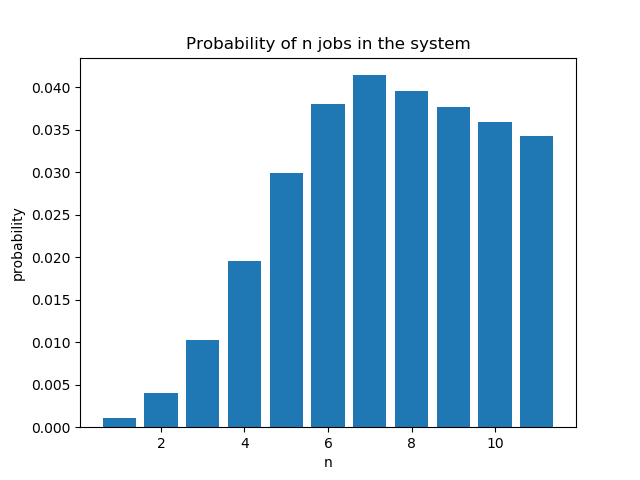
\includegraphics[scale=0.7]{/home/simon/Documents/ETH/asl/asl-fall17-project/Scripts/exp7/nJobsInSystem2.png}
\end{center} 
The system is now clearly used at its full rate, but the calculated statistics don't correspond as much to what we could observe in the middleware.
\\However, the model is able to predict that close to this arrival rate, the time in queue and the number of jobs in queue grows bigger and becomes the bottleneck of the system. In fact, when looking at the collected statistics for a one step higher workload (8 VC), we see that the number of jobs in the queue has been measured to be 12.27, and the queuing time to be 5.27 msec, which would correspond to the above stats. The reason why this model is only able to predict a given trend \underline{around} this workload is because the calculations become very volatile around a ratio of 1, and thus the numbers inputed in the model need to be very accurate which is not the case in our middleware. 
\\
For example, the inputed number for the service time and the arrival rate for 4 virtual clients were respectively 3036419ns and 2513 requests/second, whereas the numbers for 8 virtual clients are 3080518ns and 2605 requests/second, which we can see are very close to each other. However, the second configuration leads to a slightly unstable system (ratio = 1.002), and the first configuration a slightly stable configuration (ratio = 0.97). Knowing that the inputs for the two configurations are very similar, and that an error has to be taken into account in the measurements, it is reasonable to compare the outputed calculations of the 1st configuration with the collected statistics for the 2nd configuration:
 \begin{center}

		\begin{tabular}{|c|c|c|c|c|c|}
			  \hline
			  \textbf{P0} & \textbf{Jobs in system} & \textbf{Jobs in queue} & \textbf{response time[ms]} & \textbf{time in queue[ms]}\\
			  \hline
			  0.0001  & 18.52 & 10 & 3.05 & 4.33 \\
			  - & - & 12.27  & 3.081 & 5.21 \\
			  \hline
		\end{tabular}
 \end{center}
Now we are able to see that the calculated outputs correspond very well to the collected statistics.
\\\\
To conclude this part, we see that the M/M/m model is a much more suitable model for our middleware system than the M/M/1 model. When using the M/M/m model in a clearly underused configuration, the calculations are very close to the observed statistics. However, the M/M/m model outputs become very volatile when the traffic intensity (the ratio) grows close to 1, and thus, very precise statistics need to be inputed in the model to get corresponding statistics. This is not possible with our collected statistics. However it is possible to predict trends around a certain workload as seen previously. When being in a saturated configuration, the ratio grows systematically slightly over 1 due to some imprecisions and the model is not able to predict the correct values anymore. \footnote{More configurations have been tested here and lead to the same conclusion. To test more configurations, just choose a stable workload, and run the script \textit{mmm} found in the Scripts folder of experience 7, by putting the arrival rate, service time and number of worker threads to the good values}.  

\subsection{Network of Queues}
For this last part we are modelling our system with a network of queue and trying to see how some operationnal laws apply to it. We model our network of queue in the following way:
\begin{center} 
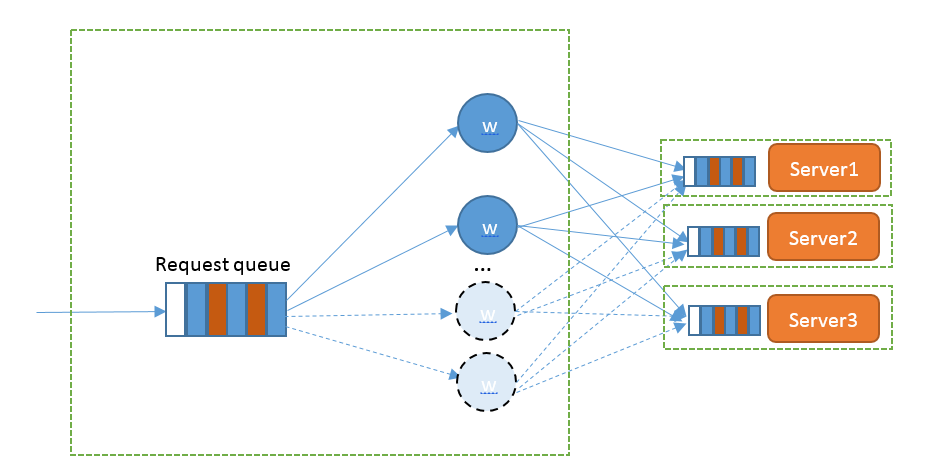
\includegraphics[scale=0.65]{/home/simon/Documents/ETH/asl/asl-fall17-project/Scripts/exp7/conf1.PNG}
\end{center} 
The request queue and the worker threads are modelled as an M/M/m queue, whereas the queues at the different servers are M/M/1. As we discussed in the last section, an M/M/m model is the most accurate way to design the first part of the system. Since all the memcached servers are independent, one M/M/1 queue per server is what makes the most sense. 
\\
In our system, this network of queue will only confirm the informations gathered about the system through this report: every request goes into the same queue, and is treated by the same pool of worker threads. As discussed in the \textit{System Overview} part, using a java \textit{ThreadPoolExecutor} will use the worker threads equally as soon as they are free. Moreover, when looking at the service time for the different threads\footnote{see any file from experiment 3}, we observe that they are all extremely close, which is not a surprise since every thread has to execute the exact same request. In consequence, this means that every worker thread is visited the same. 
The servers are also used at the same amount, since for a set operation, the request is being sent to every server, and that for a get request, the get operations are sent to a single server in a round-robin fashion.    
\\\\
This design enables us to compare the utilization of the request queue and the different worker threads with the utilization of the servers. We first calculate the different values in a generic way, by adopting the following naming convention :
\begin{itemize}
\item an index i or j: refers to a single component
\item X [req/sec]: throughput of the system
\item m: number of worker threads
\item S [ms]: service time
\item Q [ms]: queuing time
\item \(\epsilon \): parsing time (which is small)
\end{itemize}  
We start with the throughput per device by using the following formula: 
\[Xi = X*Vi\]
 \begin{center}

		\begin{tabular}{|c|c|c|}
			  \hline
			  \textbf{Device} & \textbf{Visit ratio} & \textbf{Throughput} \\
			  \hline
			  worker thread i  & 1/m & X/m \\
			  server i & 1/3 & X/3   \\
			  \hline
		\end{tabular}
 \end{center}
and thus the utilization for each device, given by:
\[Ui = Xi*Si\]
yields:
  \begin{center}

		\begin{tabular}{|c|c|c|c|}
			  \hline
			  \textbf{Device} & \textbf{Throughput} & \textbf{Service time} & \textbf{Utilization} \\
			  \hline
			  worker thread i  &X/m  & S+Q  &(X/m)$\cdot$(S+Q)\\
			  server j & X/3 & S-\(\epsilon \) &(X/3)$\cdot$(S-\(\epsilon \))  \\
			  \hline
		\end{tabular}
 \end{center}
Now we can follow this formula and find the different utilizations per device. We are using the configuration with one middleware and a read-only workload, 32 middleware threads and 2 virtual clients. The values corresponding to this configuration are:\footnote{files from exp3, normal, ratio 0:1 or 1:0, mw01, repetition 1} 
\begin{itemize}
\item X: 822
\item m: 32
\item S: 2.37
\item Q: 0.162745
\item \(\epsilon \): 0.009322
\end{itemize}
which gives (note that a small conversion is beeing made to have \textit{ms} both for throughput and times):
  \begin{center}
		\begin{tabular}{|c|c|c|c|}
			  \hline
			  \textbf{Device} & \textbf{Throughput} & \textbf{Service time} & \textbf{Utilization} \\
			  \hline
			  worker thread i  &26  & 2.53  &0.0658\\
			  server j & 274 & 2.36 &0.646  \\
			  \hline
		\end{tabular}
 \end{center}
We see that the utilization of the servers is 10 times as high than the utilization of the worker threads. This is of course because the middleware is underused with only 2 virtual clients. We now repeat the same tests with 16 virtual clients, 8 middleware threads and a write-only workload:
\begin{itemize}
\item X: 3222
\item m: 8
\item S: 2.48
\item Q: 4.95
\item \(\epsilon \): 0.007065
\end{itemize}
which leads to:
\begin{center}
		\begin{tabular}{|c|c|c|c|}
			  \hline
			  \textbf{Device} & \textbf{Throughput} & \textbf{Service time} & \textbf{Utilization} \\
			  \hline
			  worker thread i  &402  & 7.43  &2.986\\
			  server j & 1074 & 2.48 &2.666 \\
			  \hline
		\end{tabular}
 \end{center}
The statistics start now to show what we saw about the bottleneck of our system. One unique worker thread combined with the request queue has the same utilization than one server (And there are 8/3 more threads than servers!). By taking one step a higher workload (32 virtual clients), this claim can be proved:
\begin{itemize}
\item X: 3169
\item m: 8
\item S: 2.52
\item Q: 15.2
\item \(\epsilon \): 0.007065
\end{itemize}
which is:
\begin{center}
		\begin{tabular}{|c|c|c|c|}
			  \hline
			  \textbf{Device} & \textbf{Throughput} & \textbf{Service time} & \textbf{Utilization} \\
			  \hline
			  worker thread i  &396  & 17.72  &7.017\\
			  server j & 1056 & 2.52 &2.661 \\
			  \hline
		\end{tabular}
\end{center}

In a second part, we are modelling the system a little bit different to isolate the request queue, and verify even more that it is the bottleneck of our system. This is, our system will be as followed:
\begin{center} 
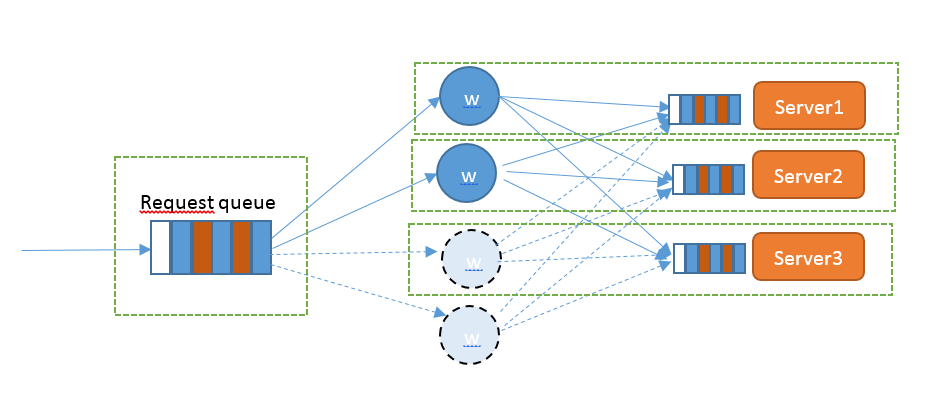
\includegraphics[scale=0.65]{/home/simon/Documents/ETH/asl/asl-fall17-project/Scripts/exp7/conf2.PNG}
\end{center} 
The request queue is now being modelled separately from the middleware threads as an M/M/1 queue. The servers are each being modelled individually with the worker thread currently communicating with this server. This is a reasonable way of modelling our system since as we saw previously, the service time of a middleware thread apart from the waiting time for the server's response is very small. With this modelling, we calculate the following generic results applying the same operationnal laws as before:
 \begin{center}
		\begin{tabular}{|c|c|c|}
			  \hline
			  \textbf{Device} & \textbf{Visit ratio} & \textbf{Throughput} \\
			  \hline
			  request queue & 1 & X \\
			  server i & 1/3 & X/3   \\
			  \hline
		\end{tabular}
 \end{center}
 and:
 \begin{center}

		\begin{tabular}{|c|c|c|c|}
			  \hline
			  \textbf{Device} & \textbf{Throughput} & \textbf{Service time} & \textbf{Utilization} \\
			  \hline
			  request queue  &X  & Q  & Q$\cdot$X\\
			  server i & X/3 & S-\(\epsilon \) &(X/3)$\cdot$(S-\(\epsilon \))  \\
			  \hline
		\end{tabular}
 \end{center}
 When being applied to a high workload, i.e the last configuration used, we obtain the following:
 \begin{itemize}
\item X: 3169
\item m: 8
\item S: 2.52
\item Q: 15.2
\item \(\epsilon \): 0.007065
\end{itemize}
which is:
 \begin{center}

		\begin{tabular}{|c|c|c|c|}
			  \hline
			  \textbf{Device} & \textbf{Throughput} & \textbf{Service time} & \textbf{Utilization} \\
			  \hline
			  request queue  &3169  & 15.2  &48.168 \\
			  server i & 1056 & 2.52 &2.661 \\
			  \hline
		\end{tabular}
 \end{center}
 The utilization of the request queue is now 18 times higher than the servers. For the previous modelling, the fact that we integrated the worker threads with the request queue to model a single M/M/m model attenuated this factor. But for this modelling, the bottleneck is definitely confirmed to be the request queue. 
 \\
 \\
 Finally, we want to have a quick look at a very important operationnal law, namely Little's law. Recall that Little's law is given by: 
 \[Length Of Queue = arrival Rate \cdot response Time\]
 This law can be verified in our system by using for example the configuration used lately, we then have:
 \begin{itemize}
\item arrival rate: 3.169 requests/ms
\item m: 8
\item S: 2.52 
\item Q: 15.2
\end{itemize}
which gives a queue length of 56, which is relatively close to the measured statistics (48). 
 
 
\end{document}
\grid
\grid
